\documentclass{beamer}
\usepackage{geometry}
\usepackage[english]{babel}
\usepackage[utf8]{inputenc}
\usepackage{amsmath}
\usepackage{amsfonts}
\usepackage{amssymb}
\usepackage{tikz}
\usetikzlibrary{quotes, angles}
\usepackage{graphicx}
\usepackage{multicol}

%\usepackage{pgfplots}
%\pgfplotsset{width=10cm,compat=1.9}
%\usepackage{pgfplotstable}

\setlength{\headheight}{26pt}%doesn't seem to fix warning

\usepackage{fancyhdr}
\pagestyle{fancy}
\fancyhf{}

%\rhead{\small{13 September 2021}}
\lhead{\small{BECA / Dr. Huson / Geometry Unit 2}}

\renewcommand{\headrulewidth}{0pt}

\title{Mathematics Class Slides}
\subtitle{Bronx Early College Academy}
\author{Christopher J. Huson PhD}
\date{18 October 2021}

\begin{document}
\frame{\titlepage}
\section[Outline]{}
\frame{\tableofcontents}

\section{3.2 Area and volume formulas, 19 October}
\frame
{
  \frametitle{Learning Target: I can name parallel lines transversal angles}
  \framesubtitle{%7.G.B.6 Solve problems involving area, volume and surface area 
  \hfill \alert{3.2 Tuesday 19 October}}
  \begin{block}{Do Now: Identify the true statements}
    \begin{multicols}{2}
    \begin{enumerate}
      \item $\angle 1 \cong \angle 2$
      \item $\angle 2 \cong \angle 4$
      \item $m\angle 1 + m\angle 4=180^\circ$
      \item $m\angle 2 + m\angle 3=90^\circ$
  \end{enumerate}
  \begin{center}
  \begin{tikzpicture}[scale=0.5, rotate=15]
    \draw [<->, thick] (0,-1.5)--(10,1.5);
    \draw [<->, thick] (2,3.5)--(7,-3.5);
    \node at (3,.4){1};
    \node at (6,-.6){3};
    \node at (5,1){2};
    \node at (4,-1){4};
  \end{tikzpicture}
  \end{center}
\end{multicols}
\end{block}
  Lesson: Parallel lines and transversal angles \\[0.25cm]
  Homework: Deltamath 3.2; Test corrections due Friday
}

\frame
  {
    \frametitle{Angle relationships}
    Review: Angle postulates and theorems you have learned. 
    \begin{enumerate}
      \item $\perp$ lines and complementary $\angle$s make $90^\circ$
      \item linear pairs add to $180^\circ$
      \item vertical $\angle$s are $\cong$
      \item definition of an angle bisector
      %\item isosceles base angle theorem
    \end{enumerate}
  }


  \frame
  {
    \frametitle{New terminology for parallel lines}
    \framesubtitle{Parallel lines are in the same plane and never intersect}
    \begin{multicols}{2}
      \begin{enumerate}
        \item \emph{parallel lines}, symbol: $\parallel$ tick marks
        \item \emph{transversal line}
        \item \emph{interior, exterior} $\angle$s
        \item \emph{same-side, alternate} $\angle$s
      \end{enumerate}
        \begin{tikzpicture}[scale=1]
        \draw [<->, thick] (3,2)--(7,2);
        \draw [<->, thick] (2,0)--(6,0);
        \draw [<->, thick] (4,-1)--(5.5,3);
        \node at (4.5,0.3) [left]{$5$};
        \node at (4.5,0.3) [right]{$6$};
        \node at (4.3,-0.3) [left]{$7$};
        \node at (4.3,-0.3) [right]{$8$};
        \node at (5.2,2) [above left]{$1$};
        \node at (5.2,2) [above right]{$2$};
        \node at (5,2) [below left]{$3$};
        \node at (5,2) [below right]{$4$};
      \end{tikzpicture}
    \end{multicols}
  }

\frame
{
  \frametitle{New theorems for parallel lines}
  \begin{multicols}{2}
    \begin{enumerate}
      \item \emph{corresponding} $\angle$s of $\parallel$ lines are $\cong$\\
        $\angle 2 \cong \angle 6$
      \item \emph{same-side interior} $\angle$s are supplementary\\
      $m\angle 3 + m\angle 5 =  180$
      \item \emph{alternate exterior} $\angle$s are $\cong$\\
      $\angle 2 \cong \angle 7$
    \end{enumerate}
      \begin{tikzpicture}[scale=1]
      \draw [<->, thick] (3,2)--(7,2);
      \draw [<->, thick] (2,0)--(6,0);
      \draw [<->, thick] (4,-1)--(5.5,3);
      \node at (4.5,0.3) [left]{$5$};
      \node at (4.5,0.3) [right]{$6$};
      \node at (4.3,-0.3) [left]{$7$};
      \node at (4.3,-0.3) [right]{$8$};
      \node at (5.2,2) [above left]{$1$};
      \node at (5.2,2) [above right]{$2$};
      \node at (5,2) [below left]{$3$};
      \node at (5,2) [below right]{$4$};
    \end{tikzpicture}
  \end{multicols}
  Hint: There are only two angle measures, the acute angles and the obtuse angles\\ (and they add to $180^\circ$)
}



\frame
{
  \frametitle{Notebook credit}
  \framesubtitle{Mastery grades 1 to 4}

  \begin{block}{Take organized notes and study them for the test Friday}
      \begin{enumerate}
        \item Well below: Few notes or no notebook
        \item Approaching expectations: Many pages of notes in a composition book. Missing several formulas and definitions.
        \item Proficient: Well organized composition book with most or all formulas and terminology easy to locate.
        \item Extending: Assesses peers and gives constructive feedback.
        \end{enumerate}\vspace{0.3cm}
        Notebook leaders: \\
        10.1 Jada, Abigail, Aiden, Nathaliah\\
        10.2 Jakia, Favour, Khudija\\
        10.3 Flora, Jefferson, Catalina

  \end{block}
}

  \frame
  {
    \frametitle{Casio fx-9750GII calculator - due Friday 1 October}
    \begin{multicols}{2}
    In the high school at BECA we use the Casio fx-9750GII.\\[5pt] 
    It is allowed on the Regents exams, SAT tests, and International Baccalaureate exams.\\[5pt]
    You may use a different calculator in Geometry if you prefer, but I recommend buying the Casio fx-9750GII.\\[5pt]
    (see me if buying a calculator is a hardship for your family)
    \includegraphics[width=3.5cm]{casio_fx-9750GII.png}
    \end{multicols}
  }

  \frame
  {
    \frametitle{Open Middle problem (fun) \\
    Use digits from 0 to 9. Using a digit no more than once.}
      The first two angle measures are complementary. The second two angles supplementary. (degrees)\\[0.75cm]
        \begin{tikzpicture}
          \draw (0,0) rectangle (1,1);
          \draw (1.25,0) rectangle (2.25,1);
          \draw (3.25,0) rectangle (4.25,1);
          \draw (4.5,0) rectangle (5.5,1);

          \draw (-1.25,-1.5) rectangle (-0.25,-0.5);
          \draw (0,-1.5) rectangle (1,-0.5);
          \draw (1.25,-1.5) rectangle (2.25,-0.5);
          \draw (3.25,-1.5) rectangle (4.25,-0.5);
          \draw (4.5,-1.5) rectangle (5.5,-0.5);
        \end{tikzpicture} \vspace{5cm} 
  }

  \section{414 Seating chart 10.1}
  \frame
  {
    \frametitle{414 Seating chart 10.1}
    \includegraphics[width=11cm]{Seating_10A-414.png}
  }

  \section{420 Seating chart 10.3}
  \frame
  {
    \frametitle{420 Seating chart 10.3}
    \begin{center}
      \includegraphics[width=11cm]{10C_seating.png}
    \end{center}
  }

\frame
{
  \frametitle{Quiz learning targets}
  \framesubtitle{7.G.B.6 Solve problems involving area, volume and surface area}

  \begin{block}{Four mastery standards}
    \begin{itemize}
    \item Solve multi-step real-life and mathematical problems posed with positive and negative rational numbers in any form (whole numbers, fractions, and decimals), using tools strategically. Apply properties of operations to calculate with numbers in any form; convert between forms as appropriate; and assess the reasonableness of answers using mental computation and estimation strategies. For example: If a woman making \$25 an hour gets a 10\% raise, she will make an additional 1/10 of her salary an hour, or \$2.50, for a new salary of \$27.50. If you want to place a towel bar 9 3/4 inches long in the center of a door that is 27 1/2 inches wide, you will need to place the bar about 9 inches from each edge; this estimate can be used as a check on the exact computation. (7.EE.B.3)
        
    \item Use facts about supplementary, complementary, vertical, and adjacent angles in a multi-step problem to write and solve simple equations for an unknown angle in a figure. (7.G.B.5)
    
    \item Solve linear equations with rational number coefficients, including equations whose solutions require expanding expressions using the distributive property and collecting like terms. (8.EE.C.7.b)
    
    \item Use geometric shapes, their measures, and their properties to describe objects. (GEO-G.MG.1)
    \end{itemize}
  \end{block}
}
  


\end{document}